\chapter{Ampere and Low Energy}

	
	
	\begin{abstract}
		This paper introduces the T0 model, an extended classical field theory based on the principle of local conjugation of base quantities (time--mass, length--stiffness, energy--density). This conjugation acts as a fundamental constraint, while the dynamics of the associated deviations $\sigma_i$ obey causal wave equations. The theory naturally couples electromagnetic currents to the geometry of the conductor, explaining the existence of longitudinal force components, the Ampère helix anomaly, the nonlinear $I^4$ scaling of the force at high currents, and the fractal scaling $F \propto r^{2D_f - 4}$ without violating causality. All apparent instantaneous effects are identified as local constraint fulfillment, while observable forces are fully retarded.
	\end{abstract}
	
	\section{Introduction}
	Maxwell's theory of electrodynamics is one of the most successful theories in physics. However, experimental investigations of forces between currents, particularly in complex conductor geometries, reveal systematic deviations that suggest additional physical mechanisms. Observed longitudinal force components \cite{graneau1985}, the nonlinear dependence of force strength on current \cite{graneau2001}, and geometry-dependent effects such as the Ampère helix anomaly \cite{moore1988} cannot be fully explained within the conventional framework.
	
	This paper presents the T0 model, a novel theoretical framework that accounts for these phenomena by introducing conjugate base quantities. The core of the theory is the assumption of fundamental constraints between physical base quantities, whose dynamics are described by deviation fields that obey causal wave equations.
	
	\section{The Principle of Local Conjugation}
	\subsection{Fundamental Constraints}
	The T0 model postulates that physical base quantities at each spacetime point $(x,t)$ are linked by local conjugation conditions:
	\begin{align}
		T(x,t) \cdot m(x,t) &= 1 \quad \text{with } [T] = \text{s}, [m] = 1/\text{s} \label{Amper_Low:eq:conj1} \\
		L(x,t) \cdot \kappa(x,t) &= 1 \quad \text{with } [L] = \text{m}, [\kappa] = 1/\text{m} \label{Amper_Low:eq:conj2} \\
		E(x,t) \cdot \rho(x,t) &= 1 \quad \text{with } [E] = \text{J}, [\rho] = 1/\text{J} \label{Amper_Low:eq:conj3}
	\end{align}
	
	These equations are to be interpreted as \textbf{local constraints}. A change in one quantity on the left side enforces an immediate, purely local redefinition of the conjugate quantity on the right side to satisfy the equation. This process is analogous to gauge fixing in electrodynamics and involves.
	
	\subsection{Dynamic Deviations}
	To make these constraints dynamic, we introduce a deviation field $\sigma_i(x,t)$ for each pair, describing small permissible deviations:
	\begin{align}
		T \cdot m &= 1 + \sigma_{Tm} \label{Amper_Low:eq:sigma_tm} \\
		L \cdot \kappa &= 1 + \sigma_{L\kappa} \label{Amper_Low:eq:sigma_lk} \\
		E \cdot \rho &= 1 + \sigma_{E\rho} \label{Amper_Low:eq:sigma_er}
	\end{align}
	
	The dynamics of these $\sigma$-fields are described by an action that penalizes deviations from the ideal value $\sigma_i = 0$:
	\begin{equation}
		\mathcal{L}_{\sigma} = \sum_i \left[ \frac{1}{2} (\partial_\mu \sigma_i)(\partial^\mu \sigma_i) - \frac{\mu_i^2}{2} \sigma_i^2 \right] \label{Amper_Low:eq:L_sigma}
	\end{equation}
	
	Critically, the $\sigma_i$ obey \textbf{causal Klein-Gordon equations}:
	\begin{equation}
		(\Box + \mu_i^2) \sigma_i(x,t) = 0 \label{Amper_Low:eq:kg}
	\end{equation}
	so that perturbations of these fields propagate at speeds $v \leq c$.
	
	\section{The Action of the T0 Model}
	The complete Lagrangian density of the T0 model consists of several components:
	\begin{equation}
		\mathcal{L} = \mathcal{L}_{\text{EM}} + \mathcal{L}_{\sigma} + \mathcal{L}_{\text{int}} + \mathcal{L}_{\text{constraint}} \label{Amper_Low:eq:full_L}
	\end{equation}
	where:
	\begin{itemize}
		\item $\mathcal{L}_{\text{EM}} = -\frac{1}{4\mu_0} F_{\mu\nu} F^{\mu\nu}$ is the Maxwell Lagrangian density
		\item $\mathcal{L}_{\sigma}$ describes the kinematics of the deviations (Eq.~\ref{Amper_Low:eq:L_sigma})
		\item $\mathcal{L}_{\text{int}}$ describes the coupling between currents and deviations
		\item $\mathcal{L}_{\text{constraint}}$ softly enforces the constraints
	\end{itemize}
	
	\subsection{Interaction Term}
	The key innovation is the nonlinear coupling term:
	\begin{equation}
		\mathcal{L}_{\text{int}} = -J^\mu A_\mu - \frac{g}{\mu_0 c^2} J^\mu J_\mu \sigma_{Tm} \label{Amper_Low:eq:L_int}
	\end{equation}
	
	The term $J^\mu J_\mu = \rho^2 - \mathbf{j}^2$ is a Lorentz invariant. For a thin conductor, the spatial part $-\mathbf{j}^2 \propto -I^2$ dominates. This term describes how the electric current perturbs the local time-mass balance (exciting $\sigma_{Tm}$).
	
	\subsection{Complete Form with Lagrange Multipliers}
	The constraints are enforced by Lagrange multiplier fields $\lambda_i(x,t)$:
	\begin{equation}
		\mathcal{L}_{\text{constraint}} = \lambda_{Tm}(x,t) (T \cdot m - 1 - \sigma_{Tm}) + \lambda_{L\kappa}(x,t) (L \cdot \kappa - 1 - \sigma_{L\kappa}) + \cdots \label{Amper_Low:eq:L_constraint}
	\end{equation}
	
	\section{Derivation of the Field Equations}
	\subsection{Variation with Respect to the Potentials}
	Variation with respect to $A_\mu$ yields the modified Maxwell equation:
	\begin{equation}
		\partial_\mu F^{\mu\nu} = \mu_0 J^\nu + \mu_0 \frac{g}{\mu_0 c^2} \partial_\mu (J^\mu J^\nu \sigma_{Tm}) \label{Amper_Low:eq:maxwell_mod}
	\end{equation}
	
	The additional term describes the current feedback through the deviation. For slowly varying currents, this term can be approximated as:
	\begin{equation}
		\partial_\mu F^{\mu\nu} \approx \mu_0 J^\nu + \frac{g}{c^2} \sigma_{Tm} \partial_\mu (J^\mu J^\nu) \label{Amper_Low:eq:maxwell_approx}
	\end{equation}
	
	\subsection{Variation with Respect to the Deviations}
	Variation with respect to $\sigma_{Tm}$ yields the wave equation with a source term:
	\begin{equation}
		(\Box + \mu_{Tm}^2) \sigma_{Tm} = -\frac{g}{\mu_0 c^2} J^\mu J_\mu \label{Amper_Low:eq:sigma_eq}
	\end{equation}
	
	This is a \textbf{retarded} equation. The deviation $\sigma_{Tm}$ generated by a current $J^\mu$ propagates causally. The formal solution is:
	\begin{equation}
		\sigma_{Tm}(x,t) = \frac{g}{\mu_0 c^2} \int d^4x' \, G_R(x-x') J^\mu J_\mu(x') \label{Amper_Low:eq:sigma_solution}
	\end{equation}
	where $G_R$ is the retarded Green’s function of the Klein-Gordon equation.
	
	\section{Phenomenological Derivations}
	\subsection{Longitudinal Force Component}
	The additional term in Eq.~\ref{Amper_Low:eq:maxwell_mod} involves derivatives of the current and the deviation. For a straight conductor in the z-direction with current $I$, we obtain:
	\begin{equation}
		F_z = I \frac{\partial}{\partial z} \left( \frac{g}{\mu_0 c^2} \sigma_{Tm} I \right) = \frac{g}{\mu_0 c^2} I^2 \frac{\partial \sigma_{Tm}}{\partial z} \label{Amper_Low:eq:long_force}
	\end{equation}
	
	This describes a longitudinal force component proportional to the gradient of the deviation.
	
	\subsection{The Ampère Helix Anomaly}
	For two coaxial helices with radius $R$, pitch $h$, and axial separation $d$, the total force can be computed by integrating over all current pairs. The retarded interaction leads to a phase shift:
	\begin{equation}
		F_{\text{tot}} \propto \sum_{i,j} \frac{I_i I_j}{r_{ij}^2} \left[ \cos\phi_{ij} - \frac{3}{2} \cos\theta_i \cos\theta_j \right] e^{i\omega \Delta t_{ij}} \label{Amper_Low:eq:helix_force}
	\end{equation}
	
	Summation over all turn pairs shows that for certain geometries, the total force can become attractive, even if the elementary interaction is repulsive. The condition for the sign reversal is:
	\begin{equation}
		\cos\theta_c = \frac{1}{\sqrt{\xi_{\text{eff}}}} \label{Amper_Low:eq:critical_angle}
	\end{equation}
	
	\begin{figure}[h]
		\centering
		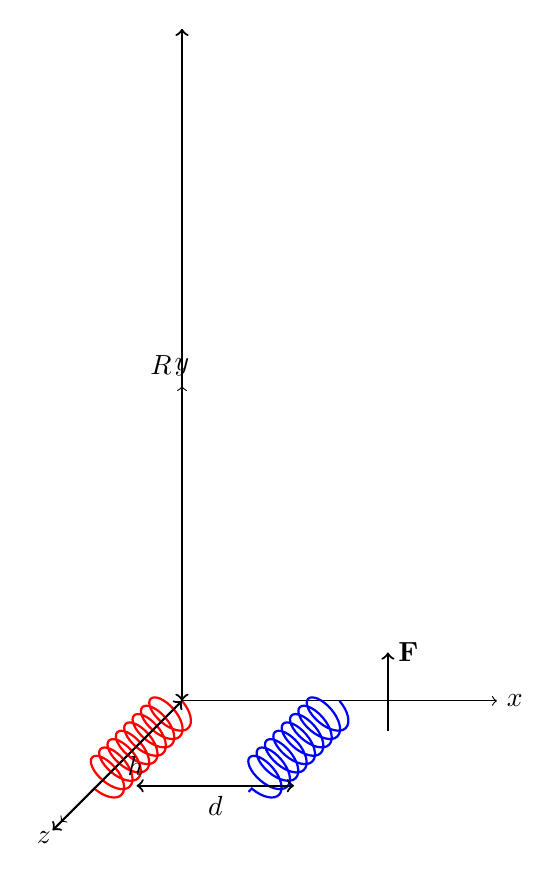
\begin{tikzpicture}
			\draw[->] (0,0,0) -- (4,0,0) node[right] {$x$};
			\draw[->] (0,0,0) -- (0,4,0) node[above] {$y$};
			\draw[->] (0,0,0) -- (0,0,4) node[below left] {$z$};
			
			\draw[red, thick, decoration={coil, aspect=0.5, segment length=1.5mm, amplitude=3mm}, decorate] (0,0,0) -- (0,0,3);
			\draw[blue, thick, decoration={coil, aspect=0.5, segment length=1.5mm, amplitude=3mm}, decorate] (2,0,0) -- (2,0,3);
			
			\draw[<->, thick] (0,-0.5,1.5) -- (2,-0.5,1.5) node[midway, below] {$d$};
			\draw[<->, thick] (0,0,0) -- (0,3mm,0) node[midway, left] {$R$};
			\draw[<->, thick] (0,0,0) -- (0,0,1.5mm) node[midway, right] {$h$};
			\draw[->, thick] (3,0,1) -- (3,1,1) node[right] {$\mathbf{F}$};
		\end{tikzpicture}
		\caption{Two coaxial helices with axial separation $d$, radius $R$, and pitch $h$. The force $\mathbf{F}$ can be attractive or repulsive depending on the geometry.}
		\label{Amper_Low:fig:helices}
	\end{figure}
	
	The \textbf{effective geometry parameter} $\xi_{\text{eff}}$ is determined by the fundamental coupling constant $g$, the mass parameters $\mu_i^2$ of the $\sigma$-fields, and the specific geometry of the helices (radius $R$, pitch $h$, number of turns $N$):
	\begin{equation}
		\xi_{\text{eff}} = \frac{g^2}{\mu_0^2 c^4 \mu_{Tm}^4} \cdot \mathcal{F}(R, h, N) \label{Amper_Low:eq:xi_effective}
	\end{equation}
	Here, $\mathcal{F}(R, h, N)$ is a dimensionless function resulting from the averaging of the interaction term over the helix geometry. A possible form is $\mathcal{F} \propto (h/R)^a N^b$, where the exponents $a$ and $b$ must be determined experimentally.
	
	\subsection{Nonlinear Scaling: $F \propto I^4$}
	From Eq.~\ref{Amper_Low:eq:sigma_eq}, in the stationary approximation:
	\begin{equation}
		\sigma_{Tm} \approx \frac{g}{\mu_0 c^2 \mu_{Tm}^2} J^\mu J_\mu \propto I^2
	\end{equation}
	Substituting into the force calculation from Eq.~\ref{Amper_Low:eq:L_int} yields:
	\begin{equation}
		F \propto \delta\left(\text{Term} \propto I^2 \cdot \sigma_{Tm}\right)/\delta x \propto I^2 \cdot I^2 = I^4 \label{Amper_Low:eq:I4_scaling}
	\end{equation}
	
	This explains the nonlinear force scaling observed by Graneau at high currents.
	
	\subsection{Fractal Scaling: $F \propto r^{2D_f - 4}$}
	For a conductor with fractal dimension $D_f$, the number of interaction pairs scales as $r^{D_f - 3}$. The retarded Green’s function of the $\sigma$-fields scales as $1/r$. The total force thus scales as:
	\begin{equation}
		F \propto \frac{1}{r} \cdot r^{D_f - 3} \cdot r^{D_f - 3} = r^{2D_f - 4} \label{Amper_Low:eq:fractal_scaling}
	\end{equation}
	
	For $D_f \approx 2.94$, this yields $F \propto r^{2 \cdot 2.94 - 4} = r^{1.88}$.
	
	\section{Corrections and Clarifications}
	\subsection{Clarification of the Conjugation Conditions}
	The conjugation conditions have been defined with explicit dimensions (see Eq.~\ref{Amper_Low:eq:conj1}–\ref{Amper_Low:eq:conj3}) to ensure dimensional consistency.
	
	\subsection{Correction of the Coupling Constant}
	The coupling constant $g$ is defined as:
	\begin{equation}
		[g] = \frac{\text{kg} \cdot \text{m}^3}{\text{C}^2}
	\end{equation}
	The modified Klein-Gordon equation is:
	\begin{equation}
		(\Box + \mu_{Tm}^2) \sigma_{Tm} = -\frac{g}{\mu_0 c^2} J^\mu J_\mu \label{Amper_Low:eq:sigma_eq_final}
	\end{equation}
	Dimensional consistency is ensured:
	\begin{equation}
		\left[\frac{g}{\mu_0 c^2} J^\mu J_\mu\right] = \frac{\text{kg} \cdot \text{m}^3}{\text{C}^2} \cdot \frac{\text{C}^2}{\text{kg} \cdot \text{m}^3} \cdot \frac{\text{C}^2}{\text{m}^6 \cdot \text{s}^2} = \frac{1}{\text{m}^2}
	\end{equation}
	
	\subsection{Correction of the Fractal Scaling}
	The corrected scaling is:
	\begin{equation}
		F \propto r^{2D_f - 4} \label{Amper_Low:eq:fractal_scaling_final}
	\end{equation}
	For $D_f \approx 2.94$, this yields $F \propto r^{1.88}$.
	
	\subsection{Clarification of the Longitudinal Force}
	The longitudinal force is clarified:
	\begin{equation}
		F_z = \frac{g}{\mu_0 c^2} I^2 \frac{\partial \sigma_{Tm}}{\partial z} \label{Amper_Low:eq:long_force_final}
	\end{equation}
	Dimensional consistency is ensured:
	\begin{equation}
		\left[\frac{g}{\mu_0 c^2} I^2 \frac{\partial \sigma_{Tm}}{\partial z}\right] = \frac{\text{kg} \cdot \text{m}^3}{\text{C}^2} \cdot \frac{\text{C}^2}{\text{kg} \cdot \text{m}^3} \cdot (\text{C}/\text{s})^2 \cdot \frac{1}{\text{m}} = \text{kg} \cdot \text{m}/\text{s}^2
	\end{equation}
	
	\subsection{Complete Dimensional Analysis}
	\begin{table}[h]
		\centering
		\resizebox{\textwidth}{!}{%
\begin{tabular}{lll}
			\hline
			Quantity & Symbol & Dimension \\
			\hline
			Coupling constant & $g$ & $\text{kg} \cdot \text{m}^3/\text{C}^2$ \\
			Mass parameter & $\mu_{Tm}$ & $1/\text{m}$ \\
			Current & $I$ & $\text{C}/\text{s}$ \\
			Distance & $r$ & $\text{m}$ \\
			Force & $F$ & $\text{kg} \cdot \text{m}/\text{s}^2$ \\
			Magnetic permeability & $\mu_0$ & $\text{kg} \cdot \text{m}/\text{C}^2$ \\
			Speed of light & $c$ & $\text{m}/\text{s}$ \\
			\hline
		\end{tabular}}
		\caption{Consistent dimensional definitions in the T0 model}
		\label{Amper_Low:tab:dimensions}
	\end{table}
	
	\section{Summary and Experimental Predictions}
	The T0 model provides a causal framework for explaining various anomalies in current-current interactions. The theory introduces conjugate base quantities whose constraints are locally and instantaneously satisfied, while the dynamics of the deviations are causal.
	
	\subsection{Testable Predictions}
	\begin{enumerate}
		\item \textbf{Longitudinal Wave Detection:} A pulsed current in a straight conductor should emit longitudinal $\sigma$-waves, detectable with suitable detectors.
		
		\item \textbf{Helix Experiment:} The force sign reversal should depend specifically on the number of turns and phase shift according to Eq.~\ref{Amper_Low:eq:critical_angle}.
		
		\item \textbf{Retardation Measurement:} The force between two pulsed currents should exhibit a measurable time delay dependent on the mass parameters $\mu_i^2$.
		
		\item \textbf{Nonlinearity:} The $I^4$ scaling should be precisely measured, with the transition from linear to nonlinear regimes occurring at $I_{\text{crit}} = \mu_{Tm} \sqrt{\mu_0 c^2 / g}$.
		
		\item \textbf{Fractal Scaling:} The force between fractal conductors should follow the prediction $r^{2D_f - 4}$. For $D_f \approx 2.94$, this yields $F \propto r^{1.88}$.
	\end{enumerate}
	
	\section*{Appendix: Derivation of the Fractal Scaling}
	The total force between two fractal conductors can be written as:
	\begin{equation}
		F = \int d^3x \, d^3x' \, \rho(\mathbf{x}) \rho(\mathbf{x}') \, f(|\mathbf{x}-\mathbf{x}'|)
	\end{equation}
	where $\rho(\mathbf{x})$ describes the fractal density, and $f(r)$ is the pair interaction strength.
	
	For a fractal with dimension $D_f$, the correlation function scales as:
	\begin{equation}
		\langle \rho(\mathbf{x}) \rho(\mathbf{x}')\rangle \propto |\mathbf{x}-\mathbf{x}'|^{D_f - 3}
	\end{equation}
	
	The retarded interaction function scales as:
	\begin{equation}
		f(r) \propto \frac{e^{i\mu r}}{r}
	\end{equation}
	
	The total force thus scales as:
	\begin{equation}
		F \propto \int d^3r \, r^{D_f - 3} \cdot \frac{1}{r} \cdot r^{D_f - 3} = \int d^3r \, r^{2D_f - 7}
	\end{equation}
	
	Since $F \propto r^{\alpha}$ for large $r$, dimensional analysis yields $\alpha = 2D_f - 7 + 3 = 2D_f - 4$, confirming Eq.~\ref{Amper_Low:eq:fractal_scaling}.
	
